\documentclass[tikz,border=8pt]{standalone}
% Shared look for every TikZ diagram. Load with % Shared look for every TikZ diagram. Load with % Shared look for every TikZ diagram. Load with \input{../../tools/tikz-style.tex}
\usepackage[T1]{fontenc}
\usepackage{lmodern}
\renewcommand{\sfdefault}{lmr}  % diagrams use the same serif as the text
\usetikzlibrary{arrows.meta, positioning, shapes.geometric, calc, fit, backgrounds}
\definecolor{cblue}{HTML}{4C78A8}
\definecolor{corange}{HTML}{F58518}
\definecolor{cgreen}{HTML}{54A24B}
\definecolor{cred}{HTML}{E45756}
\definecolor{cpurple}{HTML}{B279A2}
\definecolor{cgrey}{HTML}{6B6B6B}
\tikzset{
  every picture/.style={font=\sffamily, line width=1.2pt},
  box/.style={draw=#1, fill=#1!12, rounded corners=4pt, align=center, inner sep=7pt, minimum height=1.1cm},
  box/.default=cgrey,
  arrow/.style={-{Stealth[length=3mm]}, draw=cgrey, line width=1.4pt},
  title/.style={font=\sffamily\bfseries\Large},
  note/.style={font=\sffamily\small, text=cgrey, align=center},
}
\AtBeginDocument{\hyphenpenalty=10000 \exhyphenpenalty=10000}

\usepackage[T1]{fontenc}
\usepackage{lmodern}
\renewcommand{\sfdefault}{lmr}  % diagrams use the same serif as the text
\usetikzlibrary{arrows.meta, positioning, shapes.geometric, calc, fit, backgrounds}
\definecolor{cblue}{HTML}{4C78A8}
\definecolor{corange}{HTML}{F58518}
\definecolor{cgreen}{HTML}{54A24B}
\definecolor{cred}{HTML}{E45756}
\definecolor{cpurple}{HTML}{B279A2}
\definecolor{cgrey}{HTML}{6B6B6B}
\tikzset{
  every picture/.style={font=\sffamily, line width=1.2pt},
  box/.style={draw=#1, fill=#1!12, rounded corners=4pt, align=center, inner sep=7pt, minimum height=1.1cm},
  box/.default=cgrey,
  arrow/.style={-{Stealth[length=3mm]}, draw=cgrey, line width=1.4pt},
  title/.style={font=\sffamily\bfseries\Large},
  note/.style={font=\sffamily\small, text=cgrey, align=center},
}
\AtBeginDocument{\hyphenpenalty=10000 \exhyphenpenalty=10000}

\usepackage[T1]{fontenc}
\usepackage{lmodern}
\renewcommand{\sfdefault}{lmr}  % diagrams use the same serif as the text
\usetikzlibrary{arrows.meta, positioning, shapes.geometric, calc, fit, backgrounds}
\definecolor{cblue}{HTML}{4C78A8}
\definecolor{corange}{HTML}{F58518}
\definecolor{cgreen}{HTML}{54A24B}
\definecolor{cred}{HTML}{E45756}
\definecolor{cpurple}{HTML}{B279A2}
\definecolor{cgrey}{HTML}{6B6B6B}
\tikzset{
  every picture/.style={font=\sffamily, line width=1.2pt},
  box/.style={draw=#1, fill=#1!12, rounded corners=4pt, align=center, inner sep=7pt, minimum height=1.1cm},
  box/.default=cgrey,
  arrow/.style={-{Stealth[length=3mm]}, draw=cgrey, line width=1.4pt},
  title/.style={font=\sffamily\bfseries\Large},
  note/.style={font=\sffamily\small, text=cgrey, align=center},
}
\AtBeginDocument{\hyphenpenalty=10000 \exhyphenpenalty=10000}

\begin{document}
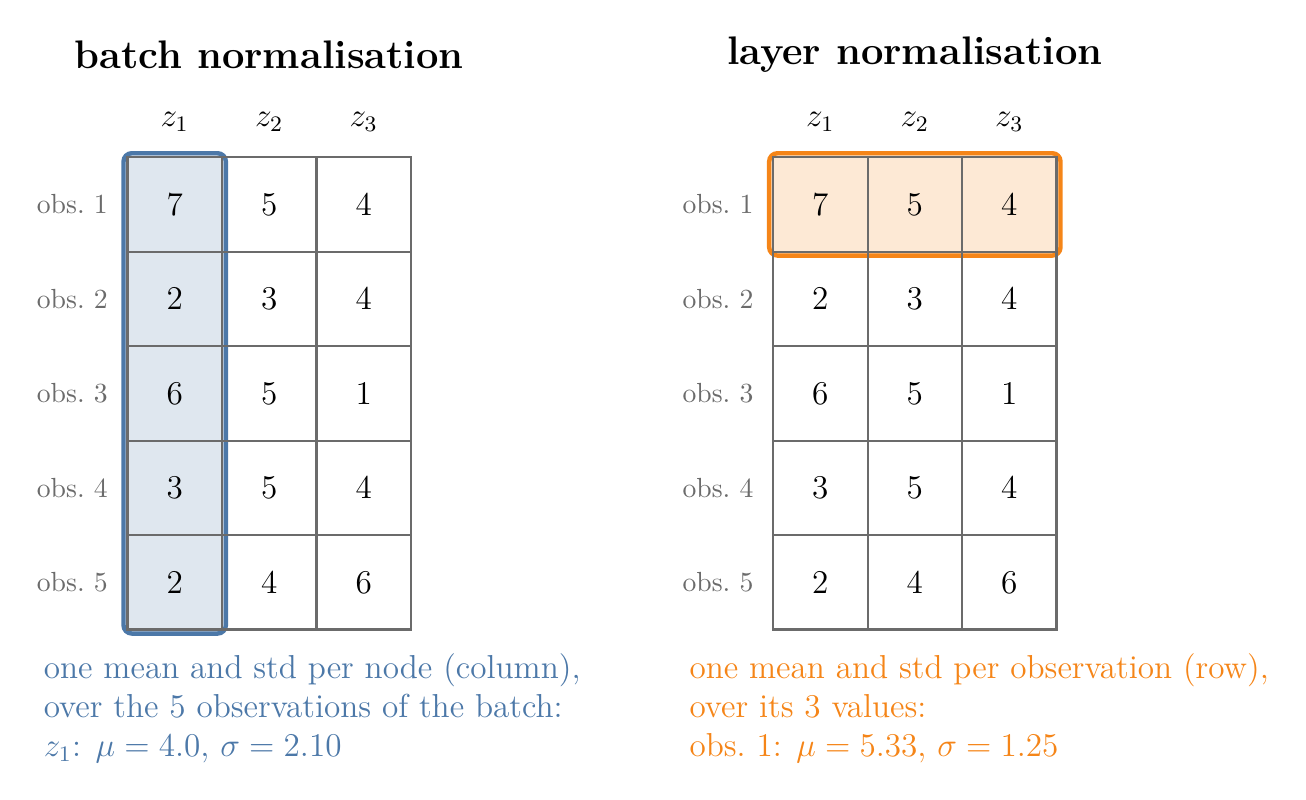
\begin{tikzpicture}[every node/.append style={font=\sffamily\large}]
  \foreach \panel/\x/\name in {0/0/batch normalisation, 1/8.2/layer normalisation} {
    \begin{scope}[xshift=\x cm]
      % highlight: column z1 for batch norm, row 1 for layer norm
      \ifnum\panel=0
        \fill[cblue!18, draw=cblue, line width=1.6pt, rounded corners=3pt] (-0.05,0.05) rectangle (1.25,-6.05);
      \else
        \fill[corange!18, draw=corange, line width=1.6pt, rounded corners=3pt] (-0.05,0.05) rectangle (3.65,-1.25);
      \fi
      \foreach \j/\h in {0/z_1,1/z_2,2/z_3} \node at (\j*1.2+0.6,0.45) {$\h$};
      \foreach \row [count=\i from 0] in {{7,5,4},{2,3,4},{6,5,1},{3,5,4},{2,4,6}} {
        \node[note, font=\sffamily] at (-0.7,-\i*1.2-0.6) {obs.\ \pgfmathparse{int(\i+1)}\pgfmathresult};
        \foreach \v [count=\j from 0] in \row {
          \node[draw=cgrey, minimum size=1.2cm, line width=0.8pt] at (\j*1.2+0.6,-\i*1.2-0.6) {$\v$};
        }
      }
      \node[title] at (1.8,1.3) {\name};
    \end{scope}
  }
  \node[note, text=cblue, font=\sffamily\large, align=left, anchor=west] at (-1.2,-7.0)
    {one mean and std per node (column),\\over the 5 observations of the batch:\\$z_1$: $\mu = 4.0$, $\sigma = 2.10$};
  \node[note, text=corange, font=\sffamily\large, align=left, anchor=west] at (7.0,-7.0)
    {one mean and std per observation (row),\\over its 3 values:\\obs.\ 1: $\mu = 5.33$, $\sigma = 1.25$};
\end{tikzpicture}
\end{document}
